%%%%%%%%%%%%%%%%%%
% Based on https://github.com/jdavis/latex-homework-template
%%%%%%%%%%%%%%%%%%

\documentclass{article}

\usepackage{fancyhdr}
\usepackage{extramarks}

\usepackage{amsmath}
\usepackage{amsthm}
\usepackage{amsfonts}

\usepackage{tikz}
\usepackage[plain]{algorithm}
\usepackage{algpseudocode}

\usetikzlibrary{automata,positioning}

\usepackage{wrapfig}

\usepackage{lipsum}

%for urls
\usepackage{hyperref}
\hypersetup{
	colorlinks = true,
	linkcolor = teal,
	anchorcolor = teal,
	citecolor = teal,
	filecolor = teal,
	urlcolor = teal
}

\usepackage{booktabs, tabularx}
\usepackage{stfloats}

%%%%%% Basic Document Settings %%%%%%%%%

\topmargin=-0.45in
\evensidemargin=0in
\oddsidemargin=0in
\textwidth=6.5in
\textheight=9.0in
\headsep=0.25in

\linespread{1.1}

%%%%%%%%%%%%%%%%%% Homework Details %%%%%%%%%%%%%%%
% University Seal
% Title
% Due date
% University
% Class
% Instructor
% Author
% Author ID 
\newcommand{\hmwkSeal}{images/logo.png}
\newcommand{\hmwkTitle}{Homework Set\ \#17}
\newcommand{\hmwkDueDate}{March 14, 3141}
\newcommand{\hmwkClass}{Course Title (CS-3.14) }
\newcommand{\hmwkClassInstructor}{Professor Augustin-Louis Cauchy}
\newcommand{\hmwkUniversity}{University of Crete \\Department of Computer Science}
\newcommand{\hmwkAuthorName}{John Doe}
\newcommand{\hmwkAuthorID}{ID XXXX}


%fancyhdr
\pagestyle{fancy}
\lhead{\hmwkAuthorName\ (\hmwkAuthorID)} %left head
%\chead{\hmwkClass\ \hmwkTitle} %center head
%\rhead{\date{\today}} %right head
\rhead{\hmwkClass\ \hmwkTitle} 
\lfoot{\lastxmark}
\cfoot{\thepage}

\renewcommand\headrulewidth{0.4pt}

% Create Problem Sections %

\newcommand{\enterProblemHeader}[1]{
	\nobreak\extramarks{}{Problem \arabic{#1} continued on next page\ldots}\nobreak{}
	\nobreak\extramarks{Problem \arabic{#1} (continued)}{Problem \arabic{#1} continued on next page\ldots}\nobreak{}
}

\newcommand{\exitProblemHeader}[1]{
	\nobreak\extramarks{Problem \arabic{#1} (continued)}{Problem \arabic{#1} continued on next page\ldots}\nobreak{}
	\stepcounter{#1}
	\nobreak\extramarks{Problem \arabic{#1}}{}\nobreak{}
}

\setcounter{secnumdepth}{0}
\newcounter{partCounter}
\newcounter{exerciseCounter}
\setcounter{exerciseCounter}{1}
\nobreak\extramarks{Problem \arabic{exerciseCounter}}{}\nobreak{}

% Homework Problem Environment %
% This environment takes an optional argument. When given, it will adjust the problem counter. This is useful for when the problems given for your
% assignment aren't sequential. See the last 3 problems of this template for an example.
%

\newcommand{\enterExerciseHeader}[1]{
	\nobreak\extramarks{}{Exercise \arabic{#1} continued on next page\ldots}\nobreak{}
	\nobreak\extramarks{Exercise \arabic{#1} (continued)}{Exercise \arabic{#1} continued on next page\ldots}\nobreak{}
}

\newcommand{\exitExerciseHeader}[1]{
	\nobreak\extramarks{Exercise \arabic{#1} (continued)}{Exercise \arabic{#1} continued on next page\ldots}\nobreak{}
	\stepcounter{#1}
	\nobreak\extramarks{Exercise \arabic{#1}}{}\nobreak{}
}

\newenvironment{Exercise}[1][-1]{
	\ifnum#1>0
	\setcounter{exerciseCounter}{#1}
	\fi
	\section{Exercise \arabic{exerciseCounter}}
	\setcounter{partCounter}{1}
	\enterExerciseHeader{exerciseCounter}
}{
	\exitExerciseHeader{exerciseCounter}
}

% Title Page %
\title{
	\centering
	\includegraphics[height=1.5in]{\hmwkSeal}
	
	\vspace{1in}
	\textmd{\textbf{\hmwkClass\ \hmwkTitle}}\\
	
	\normalsize\vspace{0.1in}\small{Due\ on\ \hmwkDueDate}\\
	
	\vspace{0.1in}
	\large{\textit{\hmwkClassInstructor}} \\
	\vspace{0.5in}
	
	\large{\hmwkUniversity}
	
	\vspace{3in}
	
	\author{\textbf{\hmwkAuthorName} (\hmwkAuthorID)}
	\date{\today}
}

% Various Helpers %
\newcommand{\alg}[1]{\textsc{\bfseries \footnotesize #1}}
% For derivatives
\newcommand{\deriv}[1]{\frac{\mathrm{d}}{\mathrm{d}x} (#1)}
% For partial derivatives
\newcommand{\pderiv}[2]{\frac{\partial}{\partial #1} (#2)}
% Integral dx
\newcommand{\dx}{\mathrm{d}x}
\newcommand{\E}{\mathbb{E}}
\newcommand{\Var}{\mathrm{Var}}
\newcommand{\Cov}{\mathrm{Cov}}
\newcommand{\Bias}{\mathrm{Bias}}

\def\code#1{\texttt{#1}}

%for code listings
\usepackage{listings}
\usepackage{xcolor}

\definecolor{codegreen}{rgb}{0,0.6,0}
\definecolor{codegray}{rgb}{0.5,0.5,0.5}
\definecolor{codepurple}{rgb}{0.58,0,0.82}
\definecolor{backcolour}{rgb}{0.99,0.99,0.99}

\lstdefinestyle{mystyle}{
	backgroundcolor=\color{backcolour},   
	commentstyle=\color{codegreen},
	keywordstyle=\color{magenta},
	numberstyle=\tiny\color{codegray},
	stringstyle=\color{codepurple},
	basicstyle=\ttfamily\footnotesize,
	breakatwhitespace=false,         
	breaklines=true,                 
	captionpos=b,                    
	keepspaces=true,                 
	numbers=left,                    
	numbersep=5pt,                  
	showspaces=false,                
	showstringspaces=false,
	showtabs=false,                  
	tabsize=2
}

\lstset{style=mystyle}

\begin{document}
	
	\maketitle
	
	\pagebreak
	
	\begin{Exercise}
    Give an appropriate positive constant $c$ such that $f(n) \leq c \cdot g(n)$ for all $n > 1$.

    \begin{enumerate}
        \item $f(n) = n^2 + n + 5$, $g(n) = 3n^2$
        \item $f(n) = n\sqrt{n} + n^2$, $g(n) = n^2$
        \item $f(n) = n^2 - n$, $g(n) = n^2 / 2$
    \end{enumerate}

    \textbf{Solution} \\


    \textbf{Part One}

    \[
        \begin{split}
            n^2 + n + 5 &=
            \\
            &\leq n^2 + n^2 + n^2
            \\
            &= 3n^2
            \\
            &\leq c \cdot 3n^2
        \end{split}
    \]

    choose $c = 1$.
    \\

    \textbf{Part Two}

    \[
        \begin{split}
            n\sqrt{n} + n^2 &=
            \\
            &= n^{3/2} + n^2
            \\
            &\leq n^{4/2} + n^2
            \\
            &= 2n^2
            \\
            &\leq c \cdot n^2
        \end{split}
    \]

    choose $c = 2$.
    \\

    \textbf{Part Three}

    \[
        \begin{split}
            n^2 - n &=
            \\
            &\leq n^2
            \\
            &\leq c \cdot \frac{n^2}{2}
        \end{split}
    \]

    again choose $c = 2$.

\end{Exercise}

\pagebreak

\begin{Exercise}
    Let $\Sigma = \{0, 1\}$. Construct a DFA $A$ that recognizes all binary numbers with even number of ones. \\
    
    \textbf{Solution} \\

    Let $\mathcal{A} = (Q, \Sigma, \delta, q_0, F)$ be the desired automaton, and let $Q = \left\{ q_0, q_1 \right\}$ where state $q_0$ corresponds to a binary number with even number of ones and $q_1$ the vase of odd number of ones. We obviously have $\Sigma = \left\{ 0,1 \right\}$ and $F=\left\{ q_0 \right\}$. 

    \begin{figure}[h]
        \centering
        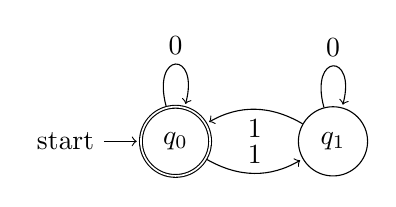
\begin{tikzpicture}[shorten >=1pt,node distance=2cm,on grid,auto]
            \node[state, accepting, initial] (q_0)   {$q_0$};
            \node[state] (q_1) [right=of q_0] {$q_1$};
            \path[->]
                (q_0)
                    edge [loop above] node {0} (q_0)
                    edge [bend right=+30] node {1} (q_1)
                (q_1)
                    edge [loop above ] node {0} (q_1)
                    edge [bend left=-30] node {1} (q_0);
        \end{tikzpicture}
        \caption{The DFA $\mathcal{A}$}
        \label{fig:multiple5}
    \end{figure}

If $A$ is in state $q_0$, inputting 1 transists to state $q_1$, while by having even number of ones (state $q_0$), inputting 1 does not result in a change of state etc, as in Figure~\ref{fig:multiple5}. Hence the transition matrix of $\delta$ is 

    \begin{table}[ht]
        \centering
        \begin{tabular}{c || c | c | c | c | c}
        	$\delta$
            & $0$
            & $1$  
            \\
            \hline
            $q_0$ & $q_0$ & $q_1$ \\
            $q_1$ & $q_1$ & $q_0$ \\
        \end{tabular}
    \end{table}

Therefore a word $w \in \left\{ 0,1 \right\}^{\star}$ is recognizable by $\mathcal{A}$ if-f $ \delta^\star (q_0, w) = q_0$, which is exactly when $w$ consists of an even number of ones.

\end{Exercise}

\pagebreak

\begin{Exercise}
    Write a pseudocode for the \alg{Insertion-Sort} algorithm. \\
    
    \textbf{Solution} \\
    
    \begin{algorithm}[]
        \begin{algorithmic}[1]
            \Function{Insertion-Sort}{Array A}
                \State{} $i=1$
                \While{$i < \text{length(A)}$}
                \State{} $j=i$
                \While{$j > 0$ and $A[j-1] > A[j]$}
                \State{}$\text{swap}(A[j],A[j-1])$
                \State{} $j \leftarrow j - 1$
                \EndWhile{}
                \State{} $i \leftarrow i + 1$
                \EndWhile{}
            \EndFunction{}
        \end{algorithmic}
        \caption{Insertion-Sort}
    \end{algorithm}
\end{Exercise}

\pagebreak

\begin{Exercise}
    Given a first order linear regression $Y_i = \beta_0 + \beta_1 x_i + e_i$ with $i = 1, \ldots, n$, $\E [e_i] = 0$, with $\Var [e_i] = \sigma^2_e$ and $\Cov[e_i, e_j] = 0, \forall i \neq j$, where $\epsilon_i$ is an error term. Obtain the least squares estimators (LSE) $\hat{\beta_0}$, $\hat{\beta_1}$.

    \begin{proof}

    \item We should minimize the Residual Sum of Squares (RSS):

    \[
            RSS = \sum_{i = 1}^{n} {(Y_i - \hat{Y_i})}^2 = \sum_{i = 1}^{n} {(Y_i - \hat{\beta_0} - \hat{\beta_1} x_i)}^2
    \]

    taking the partial derivatives with respect to $\hat{\beta_0}$ and $\hat{\beta_1}$ , we get:
    	
    \[
    \pderiv{
    	\hat{\beta_0}
    }{RSS}
    = -2 \sum_{i = 1}^{n} {(Y_i - \hat{\beta_0} - \hat{\beta_1} x_i)}
    \]
    
    \[
        \pderiv{
            \hat{\beta_1}
        }{RSS}
        = -2 \sum_{i = 1}^{n} {x_i (Y_i - \hat{\beta_0} - \hat{\beta_1} x_i)}
    \]
    
    which means
    
    \begin{equation}
    	\sum_{i = 1}^{n} {(Y_i - \hat{\beta_0} - \hat{\beta_1} x_i)} = 0 
    \end{equation}
    
    \begin{equation}
    	\sum_{i = 1}^{n} {Y_ix_i- \hat{\beta_0}x_i - \hat{\beta_1} x_i^2)} = 0 
    \end{equation}

    Expanding the sums and solving for $\hat{\beta_0}$ and $\hat{\beta_1}$ we obtain \[ \hat{\beta_0} = \overline{Y} - \hat{\beta_1}\overline{x} \]

    \begin{equation}
        \begin{split}
            \hat{\beta_1}
            &= \frac{
                \sum_{i=1}^{n} {x_i Y_i} - \frac{\sum_{i=1}^{n}x_i \sum_{i=1}^{n} Y_i}{n} 
            }{
                \sum_{i=1}^{n} x_i^2 - \frac{\left( \sum_{i=1}^{n} x_i \right)^2}{n}
            }
        \end{split}
    \end{equation}
    
\end{proof}
\end{Exercise}

\pagebreak

\begin{Exercise} Prove \textit{Liouville's Theorem}: Every bounded entire function in the complex plane $\mathbb{C}$ is constant (every holomorphic function $f$ for which there exists $M > 0$ such that $|f(z)| \leq M ~\forall z \in \mathbb{C}$ is constant).
	
	\begin{proof} Let $f$ be an entire function. Then it can be represented by its Taylor series around zero: 
		
		$$f(z) = \sum_{k=0}^\infty a_k z^k$$
		
		by Cauchy's integral formula:
		
		\[
		a_k = \frac{f^{(k)}(0)}{k!} = {1 \over 2 \pi i} \oint_{C_r} \frac{f( \zeta )}{\zeta^{k+1}}\,d\zeta
		\]
		
		where $C_r$ is the positively oriented circle around 0 of radius $r >0$. Suppose $f$ is bounded: i.e. there exists a positive constant $M$ such that $|f(z)| \leq M ~\forall z$. Then
		
		  \[
		\begin{split}
		| a_k | 
		&\le \frac{1}{2 \pi} \oint_{C_r} \frac{ | f ( \zeta ) | }{ | \zeta |^{k+1} } \, |d\zeta| \\
		&\le \frac{1}{2 \pi} \oint_{C_r} \frac{ M }{ r^{k+1} } \, |d\zeta| \\
		&= \frac{M}{2 \pi r^{k+1}} \oint_{C_r} |d\zeta| \\
		&= \frac{M}{2 \pi r^{k+1}} 2 \pi r \\
		&= \frac{M}{r^k} \\
		&\rightarrow 0
    	\end{split}
        \]
		
		as $r$ goes to infinity (since f is analytic on the entire compelx plane). Hence $a_k = 0 ~\forall k \geq 1$. Thus $f(z) = a _0$.
	\end{proof}
\end{Exercise}

\begin{Exercise}Prove the fundamental theorem of algebra using Liouville's Theorem. 
\end{Exercise}

\pagebreak
	
	\begin{Exercise}
		Show that any prime $p>3$ is next to a multiple of 6. \\
		
		\begin{proof}
		We equivalently show that every prime $p>3$ is either $p \equiv 1\text{mod}6$ or $p \equiv -1\text{mod}6 \equiv 5\text{mod}6$, that is, of the form $p = 6n + 1$ or $p=6n + 5$. By Euclidean division, every integer is of the form $n = 6q + r$ where $q$ is non-negative integer and $r =0,1,\ldots,5, ~r \leq q$. If $p$ is of of the form $6q$ or $6q+2$ or $6q+4$, then p is even, therefore not prime. If $p$ is of the form $6q+3$, then $q$ is divisible by 3 and greater than 3, and therefore not prime. The above leaves as the only candidates for primality greater than 3 integers of the form $p = 6q+1$ and $p = 6q+5 = 6(q+1) -1$. In fact, by Dirichlet's Theorem an arithmetic progression $an + b, ~n=1,2,\hdots$ generates infinitely many primes if-f $(a,b)=1$\footnote{\url{https://mathworld.wolfram.com/DirichletsTheorem.html}}.
	
    	\end{proof}

	\end{Exercise}

    \begin{Exercise}
    	In a bin there are 6 black socks and 4 blue socks. If you select two socks at random, find the probability that you select two socks of the same color. \\
    	
    	\textbf{Solution} \\
    	
    	Picking two socks of the same color means picking either two black or two blue socks. The probability of picking the first black sock is $6/10$ and $5/9$ for picking the second black sock due to sampling without replacement. So the probability of picking a black pair is $\frac{6}{10}*\frac{5}{9} = \frac{1}{3}$. Similarly, the probability of picking a blue pair is $\frac{2}{15}$. Total probability of picking a pair of black or red socks is $p=\frac{1}{3} + \frac{2}{15} = \frac{7}{15}$. Another solution using binomial coefficients instead of counting yields 
    	
    	\[
    	\frac{\binom{6}{2}}{\binom{10}{2}} + \frac{\binom{4}{2}}{\binom{10}{2}} = \frac{21}{45} = \frac{3}{15}
    	\]
    	
    \end{Exercise}

	% Non sequential homework problems
	\begin{Exercise}[224]
		Evaluate $\displaystyle \sum_{k=1}^{5} k^2$ and $\displaystyle \sum_{k=1}^{5} (k - 1)^2$.
	\end{Exercise}
	
	% Continue counting
	\begin{Exercise}
		Find the derivative of $f(x) = x^4 + 3x^2 - 2$.
	\end{Exercise}
	
	% Go back to where we left off
	\begin{Exercise}[9]
		Evaluate the integrals
		$\displaystyle \int_0^1 (1 - x^2) \dx$ and $\displaystyle \int_1^{\infty} \frac{1}{x^2} \dx$.
	\end{Exercise}

	\begin{Exercise}
		Find the derivative of $\alpha^{x}, ~a \in \mathbb{N}$. \\
		
		\textbf{Solution} \\
		
		Rewrite $\alpha^{x} \equiv e^{\ln \alpha^{x}}$, hence $e^{\ln \alpha^{x}} = e^{x\ln \alpha}$. Differentiating with respect to x, we obtain  
		
		\[
		\frac{d}{dx} e^{x\ln \alpha} = \ln (\alpha) e^{x\ln \alpha} = \ln (\alpha) \alpha^x
		\]
		
	\end{Exercise}
	
	\begin{Exercise}[243]
		Prove Goldbach's conjecture, that every even integer greater than 2 is the sum of two prime numbers.
	\end{Exercise}
	
	\begin{Exercise}[250] Prove the Riemann Hypothesis.
	\end{Exercise}
	
\end{document}
